\documentclass[border=5pt]{standalone}
\usepackage{fontspec}
\usepackage{unicode-math}
\setmainfont{Noto Serif}
\newfontfamily\FigureItalic{Noto Serif}
\setmathfont{STIXTwoMath-Regular.otf}
\usepackage{tikz}
\usetikzlibrary{arrows.meta,calc,patterns,decorations.pathmorphing,decorations.markings,decorations.pathreplacing,positioning,backgrounds}
\definecolor{Ink}{HTML}{000000}
\definecolor{Curve}{HTML}{000000}
\definecolor{Bzero}{HTML}{000000}
\definecolor{Bone}{HTML}{000000}
\definecolor{Btwo}{HTML}{000000}
\definecolor{Bthree}{HTML}{000000}
\definecolor{Bfour}{HTML}{000000}
\tikzset{
 ax/.style={draw=Ink,line width=.72pt,-{Latex[length=2.4mm,width=1.5mm]}},
 lev/.style={draw=Ink,line width=1.4pt,line cap=butt},
 thinlev/.style={draw=Ink,line width=.65pt,line cap=butt},
 helper/.style={draw=Ink,line width=.65pt},
 bare/.style={draw=Ink,line width=.95pt,dash pattern=on 4pt off 2.8pt},
 curve/.style={draw=Ink,line width=1.85pt,line cap=round,line join=round},
 ray/.style={draw=Ink,line width=1.0pt,-{Latex[length=2.3mm,width=1.4mm]}},
 measure/.style={draw=Ink,line width=.75pt,{Latex[length=1.9mm,width=1.2mm]}-{Latex[length=1.9mm,width=1.2mm]}},
 link/.style={draw=Ink,line width=1.0pt},
 wave/.style={draw=Ink,line width=.85pt,decorate,decoration={snake,amplitude=.33mm,segment length=2.5mm,pre length=.8mm,post length=.8mm}},
 photon/.style={draw=Ink,line width=1.0pt,-{Latex[length=2.0mm,width=1.3mm]},decorate,decoration={snake,amplitude=.4mm,segment length=2.7mm,pre length=0mm,post length=1.9mm}},
 lab/.style={text=Ink,font=\fontsize{13.5}{16}\selectfont,inner sep=2pt},
 small/.style={text=Ink,font=\fontsize{11.5}{14}\selectfont,inner sep=2pt},
 tag/.style={text=Ink,font=\fontsize{14}{17}\selectfont\FigureItalic\itshape,inner sep=2pt}}
\pagestyle{empty}

\begin{document}
% Figure 12.4; source-grounded revision.
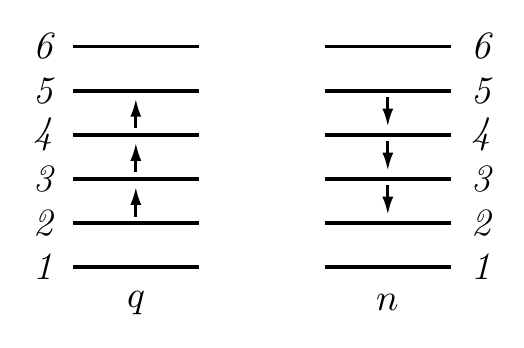
\begin{tikzpicture}[x=1cm,y=1cm]
\coordinate (q1) at (1.00000,0.00000);
\coordinate (q1L) at (0.20000,0.00000);
\coordinate (q1R) at (1.80000,0.00000);
\draw[lev] (q1L) -- (q1R);
\node[tag,anchor=east] at (0.02000,0.00000) {1};
\coordinate (q2) at (1.00000,0.56000);
\coordinate (q2L) at (0.20000,0.56000);
\coordinate (q2R) at (1.80000,0.56000);
\draw[lev] (q2L) -- (q2R);
\node[tag,anchor=east] at (0.02000,0.56000) {2};
\coordinate (q3) at (1.00000,1.12000);
\coordinate (q3L) at (0.20000,1.12000);
\coordinate (q3R) at (1.80000,1.12000);
\draw[lev] (q3L) -- (q3R);
\node[tag,anchor=east] at (0.02000,1.12000) {3};
\coordinate (q4) at (1.00000,1.68000);
\coordinate (q4L) at (0.20000,1.68000);
\coordinate (q4R) at (1.80000,1.68000);
\draw[lev] (q4L) -- (q4R);
\node[tag,anchor=east] at (0.02000,1.68000) {4};
\coordinate (q5) at (1.00000,2.24000);
\coordinate (q5L) at (0.20000,2.24000);
\coordinate (q5R) at (1.80000,2.24000);
\draw[lev] (q5L) -- (q5R);
\node[tag,anchor=east] at (0.02000,2.24000) {5};
\coordinate (q6) at (1.00000,2.80000);
\coordinate (q6L) at (0.20000,2.80000);
\coordinate (q6R) at (1.80000,2.80000);
\draw[lev] (q6L) -- (q6R);
\node[tag,anchor=east] at (0.02000,2.80000) {6};
\node[lab] at (1.00000,-0.45000) {$q$};
\coordinate (n1) at (4.20000,0.00000);
\coordinate (n1L) at (3.40000,0.00000);
\coordinate (n1R) at (5.00000,0.00000);
\draw[lev] (n1L) -- (n1R);
\node[tag,anchor=west] at (5.18000,0.00000) {1};
\coordinate (n2) at (4.20000,0.56000);
\coordinate (n2L) at (3.40000,0.56000);
\coordinate (n2R) at (5.00000,0.56000);
\draw[lev] (n2L) -- (n2R);
\node[tag,anchor=west] at (5.18000,0.56000) {2};
\coordinate (n3) at (4.20000,1.12000);
\coordinate (n3L) at (3.40000,1.12000);
\coordinate (n3R) at (5.00000,1.12000);
\draw[lev] (n3L) -- (n3R);
\node[tag,anchor=west] at (5.18000,1.12000) {3};
\coordinate (n4) at (4.20000,1.68000);
\coordinate (n4L) at (3.40000,1.68000);
\coordinate (n4R) at (5.00000,1.68000);
\draw[lev] (n4L) -- (n4R);
\node[tag,anchor=west] at (5.18000,1.68000) {4};
\coordinate (n5) at (4.20000,2.24000);
\coordinate (n5L) at (3.40000,2.24000);
\coordinate (n5R) at (5.00000,2.24000);
\draw[lev] (n5L) -- (n5R);
\node[tag,anchor=west] at (5.18000,2.24000) {5};
\coordinate (n6) at (4.20000,2.80000);
\coordinate (n6L) at (3.40000,2.80000);
\coordinate (n6R) at (5.00000,2.80000);
\draw[lev] (n6L) -- (n6R);
\node[tag,anchor=west] at (5.18000,2.80000) {6};
\node[lab] at (4.20000,-0.45000) {$n$};
\draw[ray,shorten <=2.3pt,shorten >=2.9pt] (q2) -- (q3);
\draw[ray,shorten <=2.3pt,shorten >=2.9pt] (n3) -- (n2);
\draw[ray,shorten <=2.3pt,shorten >=2.9pt] (q3) -- (q4);
\draw[ray,shorten <=2.3pt,shorten >=2.9pt] (n4) -- (n3);
\draw[ray,shorten <=2.3pt,shorten >=2.9pt] (q4) -- (q5);
\draw[ray,shorten <=2.3pt,shorten >=2.9pt] (n5) -- (n4);\end{tikzpicture}

\end{document}
